    \subsection{Introducción}
        A continuación, se analizarán los posibles riesgos, siendo estos los posibles problemas futuros que puedan tener un efecto positivo o negativo en los objetivos del proyecto, incluyendo cada uno de ellos un conjunto de causa-efectos.
        
        Para tratar mejor un riesgo, hay que tener en cuenta dos aspectos: cuál es la probabilidad de que ocurra, y cuál es el impacto que tendría en el proyecto en caso de que ocurriese.
        Una vez estimadas estas dos variables, se puede asignar una posición de ese riesgo dentro de la matriz de la figura \ref{fig:riskmatrix}.
        
        Una vez asignada su posición, se deberá priorizar todo riesgo que ocupe una posición superior a la línea de tolerancia, posiciones que poseen un color mas oscuro en la Figura \ref{fig:riskmatrix}.
        
        La matriz de la figura \ref{fig:riskmatrix} ha sido rellenada con los riesgos identificados en el Apartado \ref{sec:riesgos.identificados}, mostrando por tanto, que en este proyecto no se ha detectado ningún riesgo con el que haya que tomar una priorización sobre el resto.
        
        
        \begin{figure}[H]
            \centering
            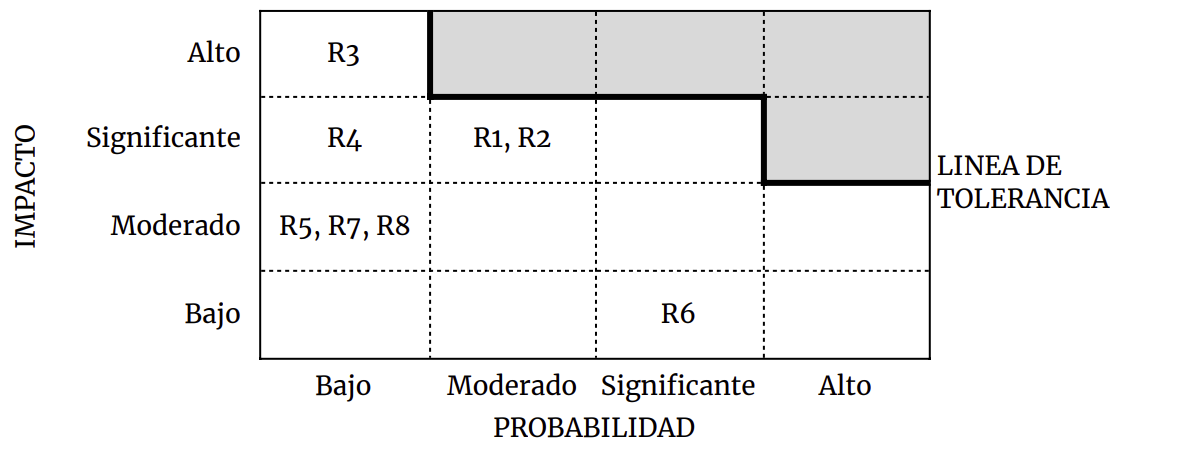
\includegraphics[width=12cm]{./img/spm/risk.matrix.png}
            \caption{Matriz de priorización de riesgos}
            \label{fig:riskmatrix}
        \end{figure}

\newpage
    \subsection{Riesgos identificados}
    \label{sec:riesgos.identificados}
        A continuación se clasifican los riesgos que pueden tener un impacto sobre el proyecto:
        %t1
        \begin{table}[H]
        \centering
        \begin{tabular}{|l|c}
        \hline
        \textbf{Riesgo}               & \multicolumn{1}{r|}{R-01}                                             \\ \hline
        \textbf{Descripción}          & \multicolumn{1}{X|}{El desarrollador puede enfermar debido a las  condiciones externas.}
        \\ \hline
        \textbf{Impacto}              & \multicolumn{1}{r|}{SIGNIFICANTE}                                             \\ \hline
        \textbf{Probabilidad}         & \multicolumn{1}{r|}{MODERADA}                                         \\ \hline
        \textbf{Plan de mitigación}   & \multicolumn{1}{X|}{Evitar acciones que atenten contra la salud. }
        \\ \hline
        \textbf{Plan de contingencia} & \multicolumn{1}{X|}{Trabajo desde casa.}
        \\ \hline
        \end{tabular}
        \caption{Riesgo 01 - Enfermedad}
        \label{table:riskill}
        \end{table}
        % t2
        \begin{table}[H]
        \centering
        \begin{tabular}{|l|c}
        \hline
        \textbf{Riesgo}               & \multicolumn{1}{r|}{R-02}                                             \\ \hline
        \textbf{Descripción}          & \multicolumn{1}{X|}{Mala planificación del proyecto.}
        \\ \hline
        \textbf{Impacto}              & \multicolumn{1}{r|}{SIGNIFICANTE}                                             \\ \hline
        \textbf{Probabilidad}         & \multicolumn{1}{r|}{MODERADA}                                         \\ \hline
        \textbf{Plan de mitigación}   & \multicolumn{1}{X|}{Reuniones cada dos semanas de seguimiento }
        \\ \hline
        \textbf{Plan de contingencia} & \multicolumn{1}{X|}{Aumentar el tiempo de trabajo hasta alcanzar lo planeado.}
        \\ \hline
        \end{tabular}
        \caption{Riesgo 02 - Planificación incorrecta}
        \label{table:malaplanif}
        \end{table}
        % t3
        \begin{table}[H]
        \centering
        \begin{tabular}{|l|c}
        \hline
        \textbf{Riesgo}               & \multicolumn{1}{r|}{R-03}                                             \\ \hline
        \textbf{Descripción}          & \multicolumn{1}{X|}{Pérdida del trabajo elaborado.}
        \\ \hline
        \textbf{Impacto}              & \multicolumn{1}{r|}{ALTO}                                             \\ \hline
        \textbf{Probabilidad}         & \multicolumn{1}{r|}{BAJA}                                         \\ \hline
        \textbf{Plan de mitigación}   & \multicolumn{1}{X|}{Utilización de varios servicios de control de versiones. }
        \\ \hline
        \textbf{Plan de contingencia} & \multicolumn{1}{X|}{Recuperar versiones más recientes.}
        \\ \hline
        \end{tabular}
        \caption{Riesgo 03 - Pérdida del trabajo}
        \label{table:riskperdida}
        \end{table}
        % t4
        \begin{table}[H]
        \centering
        \begin{tabular}{|l|c}
        \hline
        \textbf{Riesgo}               & \multicolumn{1}{r|}{R-04}                                             \\ \hline
        \textbf{Descripción}          & \multicolumn{1}{X|}{Caída de los servidores que alojan el servicio.}
        \\ \hline
        \textbf{Impacto}              & \multicolumn{1}{r|}{SIGNIFICANTE}
        \\ \hline
        \textbf{Probabilidad}         & \multicolumn{1}{r|}{BAJA}                                         \\ \hline
        \textbf{Plan de mitigación}   & \multicolumn{1}{X|}{ Usar servidores que aseguren un mínimo de disponibilidad. }
        \\ \hline
        \textbf{Plan de contingencia} & \multicolumn{1}{X|}{ Despliegue automático cuando el servidor arranque }
        \\ \hline
        \end{tabular}
        \caption{Riesgo 04 - Caída de los servidores}
        \label{table:riskperdida}
        \end{table}
        % t5
        \begin{table}[H]
        \centering
        \begin{tabular}{|l|c}
        \hline
        \textbf{Riesgo}               & \multicolumn{1}{r|}{R-05}                                             \\ \hline
        \textbf{Descripción}          & \multicolumn{1}{X|}{Rotura del equipo del dispositivo}
        \\ \hline
        \textbf{Impacto}              & \multicolumn{1}{r|}{MODERADO}                                             \\ \hline
        \textbf{Probabilidad}         & \multicolumn{1}{r|}{BAJA}                                         \\ \hline
        \textbf{Plan de mitigación}   & \multicolumn{1}{X|}{ Disponer de un mínimo de dos dispositivos. }
        \\ \hline
        \textbf{Plan de contingencia} & \multicolumn{1}{X|}{Comprar otro dispositivo.}
        \\ \hline
        \end{tabular}
        \caption{Riesgo 05 - Rotura de dispositivo}
        \label{table:riskrotura}
        \end{table}
        % t6
        \begin{table}[H]
        \centering
        \begin{tabular}{|l|c}
        \hline
        \textbf{Riesgo}               & \multicolumn{1}{r|}{R-06}                                             \\ \hline
        \textbf{Descripción}          & \multicolumn{1}{X|}{ Desconexión de la red WIFI del hogar. }
        \\ \hline
        \textbf{Impacto}              & \multicolumn{1}{r|}{BAJO}                                             \\ \hline
        \textbf{Probabilidad}         & \multicolumn{1}{r|}{SIGNIFICANTE}                                         \\ \hline
        \textbf{Plan de mitigación}   & \multicolumn{1}{X|}{ Conexión a la red a través de tarjeta SIM. }
        \\ \hline
        \textbf{Plan de contingencia} & \multicolumn{1}{X|}{ Recarga del saldo de la tarjeta SIM a través de Internet. }
        \\ \hline
        \end{tabular}
        \caption{Riesgo 06 - Desconexión de la red. }
        \label{table:riskdisconn}
        \end{table}
        % t7
        \begin{table}[H]
        \centering
        \begin{tabular}{|l|c}
        \hline
        \textbf{Riesgo}               & \multicolumn{1}{r|}{R-07}                                             \\ \hline
        \textbf{Descripción}          & \multicolumn{1}{X|}{Privatización de algún servicio.}
        \\ \hline
        \textbf{Impacto}              & \multicolumn{1}{r|}{MODERADO}                                             \\ \hline
        \textbf{Probabilidad}         & \multicolumn{1}{r|}{BAJA}                                         \\ \hline
        \textbf{Plan de mitigación}   & \multicolumn{1}{X|}{ Implementación del software adaptativa a cualquier servicio, para poder ser sustituído.
        
        Conocimiento del funcionamiento de otros servicios alternativos. }
        \\ \hline
        \textbf{Plan de contingencia} & \multicolumn{1}{X|}{ Sustitución del servicio.}
        \\ \hline
        \end{tabular}
        \caption{Riesgo 07 - Privatización de algún servicio. }
        \label{table:riskpriv}
        \end{table}


    \newpage
    \subsection{Riesgos acontecidos}
    
        Durante el transcurso del proyecto se pudo observar la aparición de ciertos riesgos:
        
        \begin{enumerate}
        
        \item \textbf{Riesgo 01 - Enfermedad}
        
        Descrito en la tabla \ref{table:riskill}, el desarrollador del sistema enfermó durante el último tramo del año.
        
        Este riesgo produjo un retraso de dos semanas en la elaboración del proyecto que el desarrollador tuvo que recuperar quitándose horas de sueño, ya que compartía este proyecto con otro trabajo externo.
        
        \item \textbf{Riesgo 02 - Mala planificación del proyecto}
        
        Descrito en la tabla \ref{table:malaplanif}, al utilizarse una planificación del proyecto mediante un modelo incremental, no se tuvo en cuenta el tiempo necesario para la escritura de la documentación formal, manteniendo una documentación informal a modo de cuaderno de bitácora donde se iban narrando los hechos.
        Este modelaje incremental hizo que se desarollasen más funciones de las que se esperaban en un principio, por lo que el periodo de escritura de la documentación aumentó notablemente, retrasando como consecuencia la finalización total del proyecto.
        
            \item \textbf{Riesgo 07 - Privatización de servicios}
            
        Descrito en la tabla \ref{table:riskpriv}, ocurrió cuando la plataforma de nuestro asistente inteligente fue comprada por Sonos. 
        
        A fecha de 31 de Enero de 2020, Snips Seeed privatizó sus servicios, bloqueando las funciones y el acceso a entrenamientos de nuestro asistente. Pese a tener analizado como posible riesgo la privatización de algún servicio, no se esperaba que la privatización fuese del asistente en general, ya que se analizó su modelo de negocio, donde se podía observar que tenía una fuerza para posicionarse como una de las primeras potencias en el mundo de los asistentes virtuales en los años venideros, ya que era el único asistente virtual capaz de trabajar sin una conexión fija a Internet. 
        
        Sonos vió también ese potencial y quiso hacerlo suyo, comprando la compañía para poseer la mejor baza de entre todos los asistentes con el fin de convertirse en los próximos años en uno de los líderes de este sector tecnológico.
        
        Gracias al plan de contingencia, y a la elaboración de un sistema que no dependa de ningun servicio específico, sino que todos los servicios implementen las funciones que el sistema requiera, el asistente podrá ser sustituido por otro de los nombrados anteriormente, posicionándose como mejor opción el asistente de Mycroft, descrito en el apartado \ref{Microft} del documento.
        
        
        \end{enumerate}